% !TeX root = ../master.tex

\lecture{9}{2026-09-22}{Makromekanik for Laminater}

\section{Makromekanik for Laminater (Klassisk Laminationsteori; CLT)} \label{sec:CLT}
En serie af lamina stakket ovenpå hinanden og limet sammen kaldes et laminat.
Laminater ses ikke som materialer men som strukturelle elementer.

Klassisk laminationsteori repræsenterer interaktionen mellem lagene i et laminat til et \textit{equivalent single layer} (ESL) rule of mixutre.
CLT kaldes også klassisk laminations-pladeteori (CLPT) og er baseret på Kirchoff-Love hypotesen, hvilket er plade-versionen af Beroulli-Euler bjælketeori.
Dette er gældende for tynde plader.

\subsection{Antagelser i CLT}
CLT er som nævnt i \Mref{sec:CLT} baseret på Kirhcoff-Love hypotesen, hvilket betyder at vi antager:
\begin{enumerate}
  \item Rette linjer, vinkelrette til midterlinjen (dvs. transverse normaler) forbliver rette efter deformation 
  \item De transverse normaler oplever ikke tøjning, dvs. den transverse normaltøjning er $\epsilon_z = 0$
  \item De transverse normaler roterer således at de forbliver vinkelrette til midterlinjen efter deformatiion, dvs. $\gamma_{xz} = 0, \gamma_{yz} = 0 \implies \tau_{xz} = 0, \tau_{yz} = 0$
\end{enumerate}
De ovenstående antagelser er vist på \Mref{fig:clt-antagelser}.


\begin{figure} [ht]
  \centering
  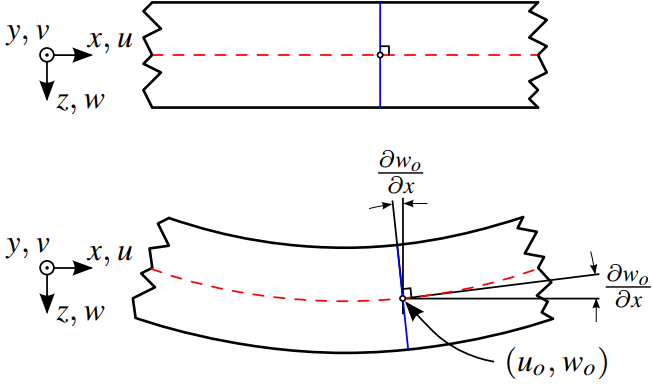
\includegraphics[width=0.5\linewidth]{./figures/clt-antagelser.png}
  \caption{Antagelser under deformation for CLT.}
  \label{fig:clt-antagelser}
\end{figure}

Ydermere antager vi lineær materialeopførsel, hvilket betyder:
\begin{enumerate}
  \item Forskydninger $u(x,y,z), v(x,y,z)$, and $w(x,y,z)$ er små ift. tykkelsen på laminatet
  \item Plantøjningerne $\epsilon_x$, $\epsilon_y$ og $\gamma_{xy}$ er små ift. 1.
\end{enumerate}


\subsection{Tøjningsforskydnings-relationen for CLT}
Tøjningsudtrykket i CLT er:
\begin{equation} \label{eq:tøjningsforskydningsclt}
  \begin{bmatrix}
    \epsilon_x\\
  \epsilon_y\\
  \gamma_{xy}\\
  \end{bmatrix} = \begin{bmatrix}
    \epsilon_{x}^{\circ}\\
  \epsilon_{y}^{\circ}\\
  \gamma_{xy}^{\circ}\\
  \end{bmatrix} + z \begin{bmatrix}
    \kappa_{x}\\
  \kappa_y\\
  \kappa_{xy}\\
  \end{bmatrix}
\end{equation}
hvor, $\epsilon_{x}^{\circ}, \epsilon_y^{\circ}$ og $\gamma_{xy}^{\circ}$ er tøjningerne ved midterlinjen og $\kappa_x$, $\kappa_y$, $\kappa_{xy}$ er krumningen (invers krumningsradius) ved midterlinjen.

\subsection{Spændings-tøjnings-relation for CLT}
Vi har allerede den generelle spændings-tøjningsrelation:
\begin{equation*}
  \begin{bmatrix}
    \sigma_x\\
  \sigma_y\\
  \tau_{xy}\\
  \end{bmatrix}_k = \begin{bmatrix}
    \overline{Q}_{11} & \overline{Q}_{12} & \overline{Q}_{16}\\
  \overline{Q}_{12} & \overline{Q}_{22} & \overline{Q}_{26}\\
  \overline{Q}_{16} & \overline{Q}_{26} & \overline{Q}_{66}\\
  \end{bmatrix}_k \begin{bmatrix}
    \epsilon_x\\
  \epsilon_y\\
  \tau_{xy}\\
  \end{bmatrix}_k
.\end{equation*}
Substitueres udtrykket i \Mref{eq:tøjningsforskydningsclt} herind fås:
\begin{equation} \label{eq:spændingstøjningsclt}
  \begin{bmatrix}
    \sigma_{x}\\
  \sigma_y\\
  \tau_{xy}\\
  \end{bmatrix}_k = \begin{bmatrix}
    \overline{Q}_{11} & \overline{Q}_{12} & \overline{Q}_{16}\\
  \overline{Q}_{12} & \overline{Q}_{22} & \overline{Q}_{26}\\
  \overline{Q}_{16} & \overline{Q}_{26} & \overline{Q}_{66}\\
  \end{bmatrix}_k \left( \begin{bmatrix}
    \epsilon_{x}^{\circ}\\
  \epsilon_y^{\circ}\\
  \gamma_{xy}^{\circ}\\
  \end{bmatrix} + z \begin{bmatrix}
    \kappa_x\\
  \kappa_y\\
  \kappa_{xy}\\
  \end{bmatrix} \right)
.\end{equation}
I \mref{eq:spændingstøjningsclt} indikerer subskriptet $k$ at der er tale om komposittens $k$'te lag.
Dette er vist på \Mref{fig:spændingstøjningsclt}. BEMÆRK: $z$-retningen regnes ALTID nedad.

\begin{figure} [ht]
  \centering
  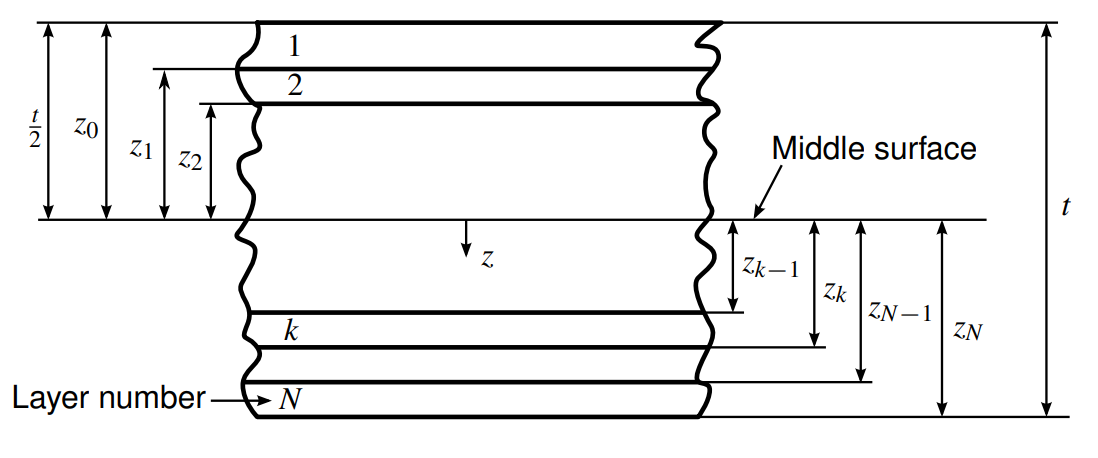
\includegraphics[width=0.7\linewidth]{./figures/spændingstøjningsclt.png}
  \caption{Figur over de forskellige lag i et laminat med $z$-retningen nedad.}
  \label{fig:spændingstøjningsclt}
\end{figure}

Det ovenstående giver eksempelvis spændings- og tøjningsfordeling samt karakteristisk modul for et laminat vist på \Mref{fig:fordelingerclt}.
Bemærk at tøjningen er kontinuert idet der ikke er skrid imellem lagene.

\begin{figure} [ht]
  \centering
  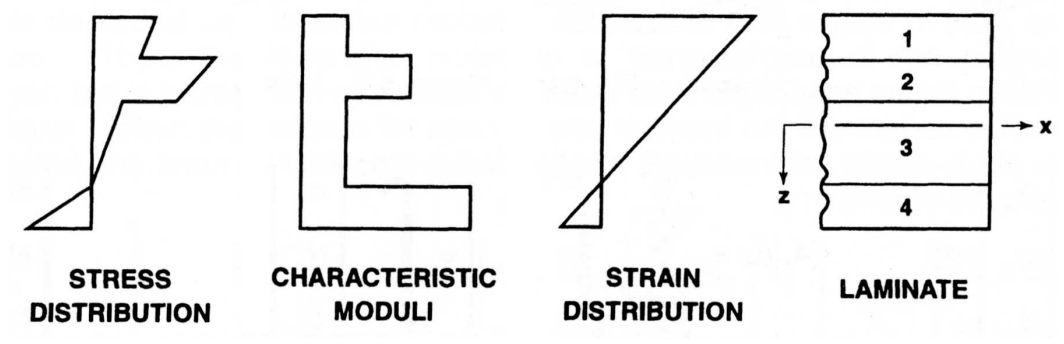
\includegraphics[width=0.6\linewidth]{./figures/fordelingerclt.png}
  \caption{Spændings- og tøjningsfordeling samt karakteristisk modul for et laminat. Reproduceret fra \citepage{jones2021mechanicscompositematerials}{195}.}
  \label{fig:fordelingerclt}
\end{figure}

\subsection{Kræfter i CLT}
Integration over alle spændinger giver de resulterende kræfter vist på \Mref{fig:cltforces}.
Dette udføres som:
\begin{equation*}
  \begin{bmatrix}
    N_x\\
  N_y\\
  N_{xy}\\
  \end{bmatrix} = \int_{-\frac{t}{2}}^{\frac{t}{2}} \begin{bmatrix}
    \sigma_x\\
  \sigma_y\\
  \tau_{xy}\\
  \end{bmatrix} \, \mathrm{d}z = \sum_{k = 1}^{N} \int_{z_{k-1}}^{z_k} \begin{bmatrix}
    \sigma_x\\
  \sigma_y\\
  \tau_{xy}\\
  \end{bmatrix}_k \, \mathrm{d}z
.\end{equation*}


\begin{figure} [ht]
  \centering
  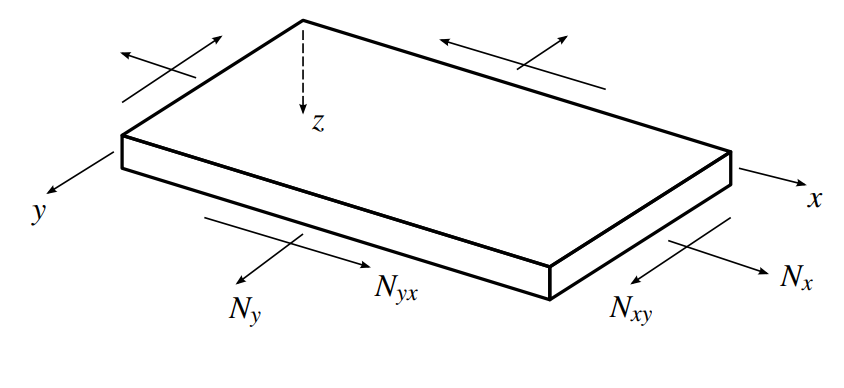
\includegraphics[width=0.5\linewidth]{./figures/cltforces.png}
  \caption{Resulterende kræfter i CLT.}
  \label{fig:cltforces}
\end{figure}

\subsection{Momenter i CLT}
De resulterende momenter findes blot som:
\begin{equation*}
  \begin{bmatrix}
    M_x\\
  M_y\\
  M_{xy}\\
  \end{bmatrix} = \int_{- \frac{t}{2}}^{\frac{t}{2}}  \begin{bmatrix}
    \sigma_x\\
  \sigma_y\\
  \tau_{xy}\\
  \end{bmatrix} z \, \mathrm{d}z = \sum_{k = 1}^{N} \int_{z_{k-1}}^{z_k} \begin{bmatrix}
    \sigma_x\\
  \sigma_y\\
  \tau_{xy}\\
  \end{bmatrix}_k z \, \mathrm{d}z
.\end{equation*}
Dette udføres med den underlige konvention for retningena af $M_x$ og $M_y$ fra \Mref{fig:cltmoments}.

\begin{figure} [ht]
  \centering
  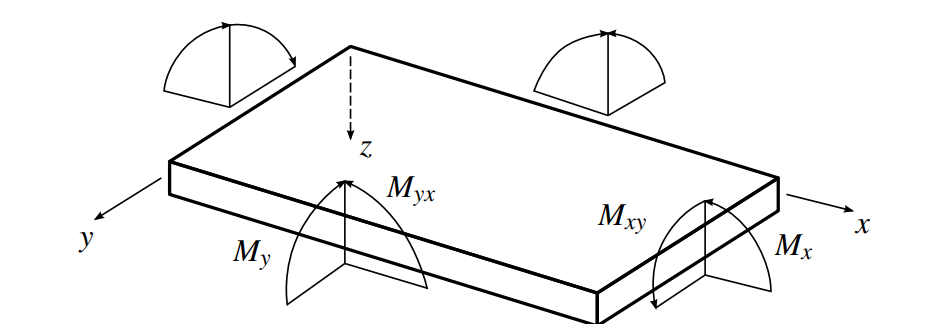
\includegraphics[width=0.5\linewidth]{./figures/cltmoments.png}
  \caption{Momenter i CLT, bemærk den underlige konvention for retningen af $M_x$ og $M_y$.}
  \label{fig:cltmoments}
\end{figure}

\subsection{ABD-Matrix for CLT}
ABD-Matricerne for CLT er:
\begin{align*}
  \begin{bmatrix}
    N_x\\
  N_y\\
  N_{xy}\\
  \end{bmatrix} &= \begin{bmatrix}
    A_{11} & A_{12} & A_{16}\\
  A_{12} & A_{22} & A_{26}\\
  A_{16} & A_{26} & A_{66}\\
  \end{bmatrix} \begin{bmatrix}
    \epsilon_x^{\circ}\\
  \epsilon_y^{\circ}\\
  \gamma_{xy}^{\circ}\\
  \end{bmatrix} + \begin{bmatrix}
    B_{11} & B_{12} & B_{16}\\
  B_{12} & B_{22} & B_{26}\\
  B_{16} & B_{26} & B_{66}\\
  \end{bmatrix} \begin{bmatrix}
    \kappa_x\\
  \kappa_y\\
  \kappa_{xy}\\
  \end{bmatrix} \\
  \begin{bmatrix}
    M_x\\
  M_y\\
  M_{xy}\\
\end{bmatrix} &= \begin{bmatrix}
  B_{11} & B_{12} & B_{16}\\
B_{12} & B_{22} & B_{26}\\
B_{16} & B_{26} & B_{66}\\
\end{bmatrix} \begin{bmatrix}
  \epsilon_x^{\circ}\\
\epsilon_y^{\circ}\\
\gamma_{xy}^{\circ}\\
\end{bmatrix} + \begin{bmatrix}
  D_{11} & D_{12} & D_{16}\\
D_{12} & D_{22} & D_{26}\\
D_{16} & D_{26} & D_{66}\\
\end{bmatrix} \begin{bmatrix}
  \kappa_x\\
\kappa_y\\
\kappa_{xy}\\
\end{bmatrix}
.\end{align*}
Hvor, $A_{ij}$ er extensions-stivhedsmatricen, $B_{ij}$ er bøjnings-extensions-stivhedsmatricen og $D_{ij}$ er bøjnings-stivhedsmatricen.
